%!TEX root=qsic2014.tex
% mainfile: qsic2014.tex

\subsection{Experiment Design}

%GREG- I stuck to using "we" here because this is the process "we" executed. Is this okay to leave this way?

All experiments were performed on GNU/Linux workstations with kernel 3.2.0-44, a 2 GHzIntel Corporation Xeon E5/Core i7
processor and  15.6 GB of main memory. The unit tests were generated in the Java programming language, for both manual
and automated tests. Figure~\ref{fig:process_diagram}  provides an overview of the test generation implementation with
edges between interacting components. First we identified ten programs
in the SF110~\cite{fraser:2012}. These
programs needed to have manually written test suites for them already to compare to the automated test suites.
Table~\ref{tbl:program_table} provides a list of the selected SF110 programs with their respective lines of code and
cyclomatic complexity.  After identifying these programs, we use the automated test tools Evosuite and Codepro to
generate test suites. We then took the manual and automated generated test suites and used several different tools to
collect the metrics. MAJOR is used find the mutation score of the program, JaCoCo is used to attain the branch coverage,
and JavaNCSS measures the lines of code and the cyclic complexity of the programs. Time to create the tests was also
recorded manually to compare Evosuite and CodePro. Time to create the manual tests was available with the SF110.

Because Evosuite uses a genetic algorithm to generate unit tests, we generated the tests for Evosuite ten times for each program. With multiple datasets, we can more accurate results with the standard deviation between mutation score, coverage, and time. CodePro uses a deterministic algorithm to generate the tests, so multiple test suite generations were not needed. With results gathered from Evosuite, CodePro, and the manually written tests, we then compared the scores based upon complexity, time to generate test suite, mutation score, lines of code, and branch coverage.

%GREG\KRISTEN - Here we talk about the graphs and error in statistical analysis. Power symbol ^ is not working for me.
%I'm assuming also we are going to want to include equations for how we calculate R^2 values and the best fit line.
%Do we need a table of results for the R^2 values?

For the graphs, we attempted to find the best fit line to accurately represent to results. It is difficult to find a truly best fit line that gives an overall statistical overlook of the data. This is due to the varying nature of both Evosuite and the manually written tests. Evosuite uses a genetic algorithm, which results in varied results for each iteration. This is why as mentioned before, we run ten generations of the test suites and calculate an average for the standard deviation. Manually written test suites are written by different developers. These varying factors result in low  R2 scores, which correlate to how well the best fit line actually represents the data. However, CodePro generated a mutation score of 0 in some cases. We removed these results for CodePro results because it skewed the data in a way that was not graphically indicative of the trends we discovered with CodePro. 

\begin{table}[!t]
\caption{Benchmark Programs and their Properties}
\label{tbl:program_table}
\resizebox{\columnwidth}{!}{%
\begin{tabular}{|l|c|c|}
\hline
\textbf{Program} & \textbf{LOC} &\textbf{Cyclomatic Complexity} \\ \hline
Netweaver                              & 17953                              & 2.82                                                \\ \hline
Inspirento                             & 1769                               & 1.76                                                \\ \hline
Jsecurity                              & 9470                               & 2.05                                                \\ \hline
Saxpath                                & 1441                               & 2.10                                                \\ \hline
Jni-inchi                              & 783                                & 2.05                                                \\ \hline
Xisemele                               & 1399                               & 1.29                                                \\ \hline
Diebierse                              & 1539                               & 1.74                                                \\ \hline
Lagoon                                 & 6060                               & 3.52                                                \\ \hline
Lavalamp                               & 1039                               & 1.50                                                \\ \hline
Jnfe                                   & 1294                               & 1.38                                                \\ \hline
\end{tabular}
}
\end{table}
%JACOB: Put in the text, not the table: "Physical lines of code calculated by JavaNCSS


\begin{figure*}[!t]
\centering
\captionsetup{justification=centering}
  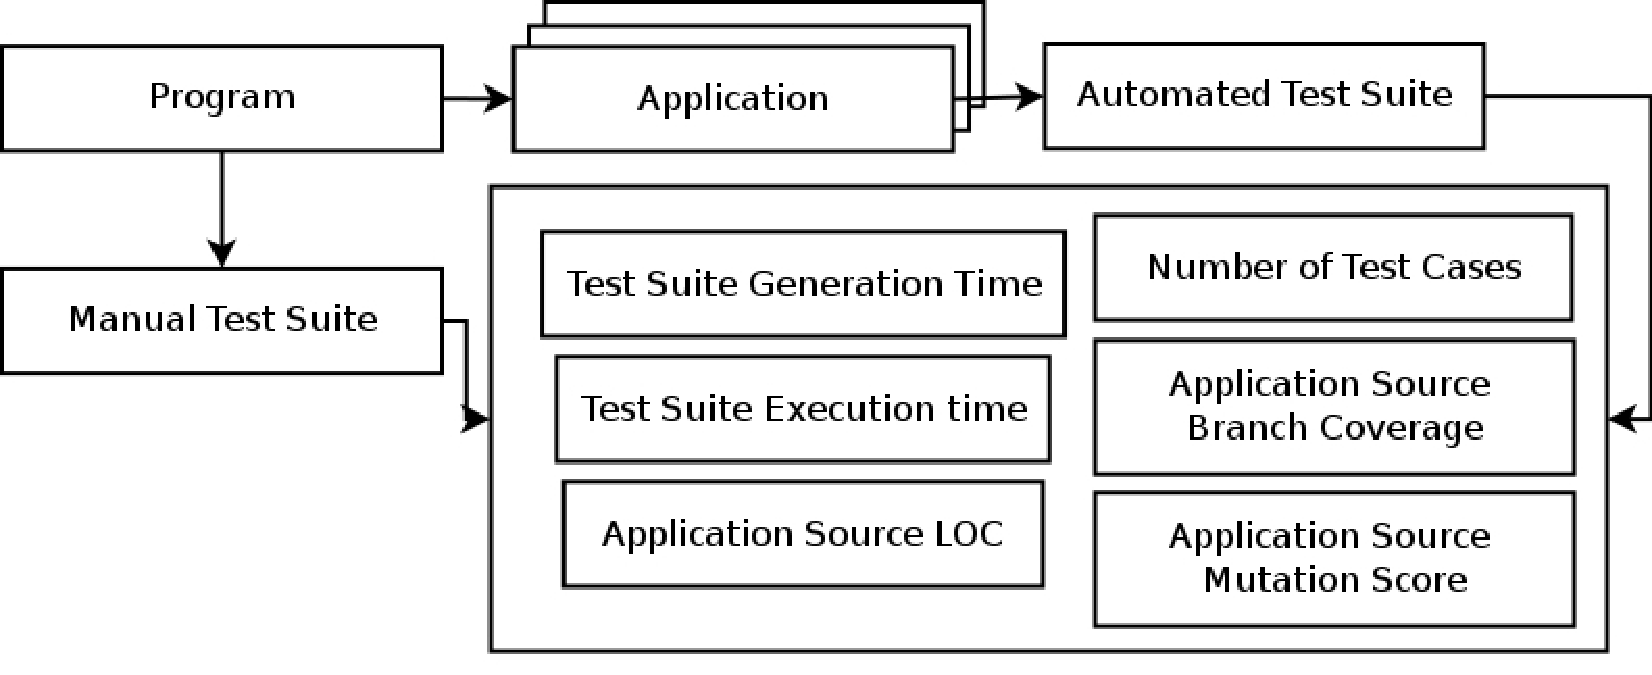
\includegraphics[width=\linewidth]{proccess_diagram.pdf}
    \caption{Test and Mutation Process}
  \label{fig:process_diagram}
\end{figure*}

